% Generated by Sphinx.
\def\sphinxdocclass{report}
\documentclass[letterpaper,10pt,english]{sphinxmanual}
\usepackage[utf8]{inputenc}
\DeclareUnicodeCharacter{00A0}{\nobreakspace}
\usepackage[T1]{fontenc}
\usepackage{babel}
\usepackage{times}
\usepackage[Bjarne]{fncychap}
\usepackage{longtable}
\usepackage{sphinx}
\usepackage{multirow}


\title{Chimaira Documentation}
\date{August 23, 2012}
\release{0.2.1}
\author{Nick Eriksson}
\newcommand{\sphinxlogo}{}
\renewcommand{\releasename}{Release}
\makeindex

\makeatletter
\def\PYG@reset{\let\PYG@it=\relax \let\PYG@bf=\relax%
    \let\PYG@ul=\relax \let\PYG@tc=\relax%
    \let\PYG@bc=\relax \let\PYG@ff=\relax}
\def\PYG@tok#1{\csname PYG@tok@#1\endcsname}
\def\PYG@toks#1+{\ifx\relax#1\empty\else%
    \PYG@tok{#1}\expandafter\PYG@toks\fi}
\def\PYG@do#1{\PYG@bc{\PYG@tc{\PYG@ul{%
    \PYG@it{\PYG@bf{\PYG@ff{#1}}}}}}}
\def\PYG#1#2{\PYG@reset\PYG@toks#1+\relax+\PYG@do{#2}}

\expandafter\def\csname PYG@tok@gd\endcsname{\def\PYG@tc##1{\textcolor[rgb]{0.63,0.00,0.00}{##1}}}
\expandafter\def\csname PYG@tok@gu\endcsname{\let\PYG@bf=\textbf\def\PYG@tc##1{\textcolor[rgb]{0.50,0.00,0.50}{##1}}}
\expandafter\def\csname PYG@tok@gt\endcsname{\def\PYG@tc##1{\textcolor[rgb]{0.00,0.25,0.82}{##1}}}
\expandafter\def\csname PYG@tok@gs\endcsname{\let\PYG@bf=\textbf}
\expandafter\def\csname PYG@tok@gr\endcsname{\def\PYG@tc##1{\textcolor[rgb]{1.00,0.00,0.00}{##1}}}
\expandafter\def\csname PYG@tok@cm\endcsname{\let\PYG@it=\textit\def\PYG@tc##1{\textcolor[rgb]{0.25,0.50,0.56}{##1}}}
\expandafter\def\csname PYG@tok@vg\endcsname{\def\PYG@tc##1{\textcolor[rgb]{0.73,0.38,0.84}{##1}}}
\expandafter\def\csname PYG@tok@m\endcsname{\def\PYG@tc##1{\textcolor[rgb]{0.13,0.50,0.31}{##1}}}
\expandafter\def\csname PYG@tok@mh\endcsname{\def\PYG@tc##1{\textcolor[rgb]{0.13,0.50,0.31}{##1}}}
\expandafter\def\csname PYG@tok@cs\endcsname{\def\PYG@tc##1{\textcolor[rgb]{0.25,0.50,0.56}{##1}}\def\PYG@bc##1{\setlength{\fboxsep}{0pt}\colorbox[rgb]{1.00,0.94,0.94}{\strut ##1}}}
\expandafter\def\csname PYG@tok@ge\endcsname{\let\PYG@it=\textit}
\expandafter\def\csname PYG@tok@vc\endcsname{\def\PYG@tc##1{\textcolor[rgb]{0.73,0.38,0.84}{##1}}}
\expandafter\def\csname PYG@tok@il\endcsname{\def\PYG@tc##1{\textcolor[rgb]{0.13,0.50,0.31}{##1}}}
\expandafter\def\csname PYG@tok@go\endcsname{\def\PYG@tc##1{\textcolor[rgb]{0.19,0.19,0.19}{##1}}}
\expandafter\def\csname PYG@tok@cp\endcsname{\def\PYG@tc##1{\textcolor[rgb]{0.00,0.44,0.13}{##1}}}
\expandafter\def\csname PYG@tok@gi\endcsname{\def\PYG@tc##1{\textcolor[rgb]{0.00,0.63,0.00}{##1}}}
\expandafter\def\csname PYG@tok@gh\endcsname{\let\PYG@bf=\textbf\def\PYG@tc##1{\textcolor[rgb]{0.00,0.00,0.50}{##1}}}
\expandafter\def\csname PYG@tok@ni\endcsname{\let\PYG@bf=\textbf\def\PYG@tc##1{\textcolor[rgb]{0.84,0.33,0.22}{##1}}}
\expandafter\def\csname PYG@tok@nl\endcsname{\let\PYG@bf=\textbf\def\PYG@tc##1{\textcolor[rgb]{0.00,0.13,0.44}{##1}}}
\expandafter\def\csname PYG@tok@nn\endcsname{\let\PYG@bf=\textbf\def\PYG@tc##1{\textcolor[rgb]{0.05,0.52,0.71}{##1}}}
\expandafter\def\csname PYG@tok@no\endcsname{\def\PYG@tc##1{\textcolor[rgb]{0.38,0.68,0.84}{##1}}}
\expandafter\def\csname PYG@tok@na\endcsname{\def\PYG@tc##1{\textcolor[rgb]{0.25,0.44,0.63}{##1}}}
\expandafter\def\csname PYG@tok@nb\endcsname{\def\PYG@tc##1{\textcolor[rgb]{0.00,0.44,0.13}{##1}}}
\expandafter\def\csname PYG@tok@nc\endcsname{\let\PYG@bf=\textbf\def\PYG@tc##1{\textcolor[rgb]{0.05,0.52,0.71}{##1}}}
\expandafter\def\csname PYG@tok@nd\endcsname{\let\PYG@bf=\textbf\def\PYG@tc##1{\textcolor[rgb]{0.33,0.33,0.33}{##1}}}
\expandafter\def\csname PYG@tok@ne\endcsname{\def\PYG@tc##1{\textcolor[rgb]{0.00,0.44,0.13}{##1}}}
\expandafter\def\csname PYG@tok@nf\endcsname{\def\PYG@tc##1{\textcolor[rgb]{0.02,0.16,0.49}{##1}}}
\expandafter\def\csname PYG@tok@si\endcsname{\let\PYG@it=\textit\def\PYG@tc##1{\textcolor[rgb]{0.44,0.63,0.82}{##1}}}
\expandafter\def\csname PYG@tok@s2\endcsname{\def\PYG@tc##1{\textcolor[rgb]{0.25,0.44,0.63}{##1}}}
\expandafter\def\csname PYG@tok@vi\endcsname{\def\PYG@tc##1{\textcolor[rgb]{0.73,0.38,0.84}{##1}}}
\expandafter\def\csname PYG@tok@nt\endcsname{\let\PYG@bf=\textbf\def\PYG@tc##1{\textcolor[rgb]{0.02,0.16,0.45}{##1}}}
\expandafter\def\csname PYG@tok@nv\endcsname{\def\PYG@tc##1{\textcolor[rgb]{0.73,0.38,0.84}{##1}}}
\expandafter\def\csname PYG@tok@s1\endcsname{\def\PYG@tc##1{\textcolor[rgb]{0.25,0.44,0.63}{##1}}}
\expandafter\def\csname PYG@tok@gp\endcsname{\let\PYG@bf=\textbf\def\PYG@tc##1{\textcolor[rgb]{0.78,0.36,0.04}{##1}}}
\expandafter\def\csname PYG@tok@sh\endcsname{\def\PYG@tc##1{\textcolor[rgb]{0.25,0.44,0.63}{##1}}}
\expandafter\def\csname PYG@tok@ow\endcsname{\let\PYG@bf=\textbf\def\PYG@tc##1{\textcolor[rgb]{0.00,0.44,0.13}{##1}}}
\expandafter\def\csname PYG@tok@sx\endcsname{\def\PYG@tc##1{\textcolor[rgb]{0.78,0.36,0.04}{##1}}}
\expandafter\def\csname PYG@tok@bp\endcsname{\def\PYG@tc##1{\textcolor[rgb]{0.00,0.44,0.13}{##1}}}
\expandafter\def\csname PYG@tok@c1\endcsname{\let\PYG@it=\textit\def\PYG@tc##1{\textcolor[rgb]{0.25,0.50,0.56}{##1}}}
\expandafter\def\csname PYG@tok@kc\endcsname{\let\PYG@bf=\textbf\def\PYG@tc##1{\textcolor[rgb]{0.00,0.44,0.13}{##1}}}
\expandafter\def\csname PYG@tok@c\endcsname{\let\PYG@it=\textit\def\PYG@tc##1{\textcolor[rgb]{0.25,0.50,0.56}{##1}}}
\expandafter\def\csname PYG@tok@mf\endcsname{\def\PYG@tc##1{\textcolor[rgb]{0.13,0.50,0.31}{##1}}}
\expandafter\def\csname PYG@tok@err\endcsname{\def\PYG@bc##1{\setlength{\fboxsep}{0pt}\fcolorbox[rgb]{1.00,0.00,0.00}{1,1,1}{\strut ##1}}}
\expandafter\def\csname PYG@tok@kd\endcsname{\let\PYG@bf=\textbf\def\PYG@tc##1{\textcolor[rgb]{0.00,0.44,0.13}{##1}}}
\expandafter\def\csname PYG@tok@ss\endcsname{\def\PYG@tc##1{\textcolor[rgb]{0.32,0.47,0.09}{##1}}}
\expandafter\def\csname PYG@tok@sr\endcsname{\def\PYG@tc##1{\textcolor[rgb]{0.14,0.33,0.53}{##1}}}
\expandafter\def\csname PYG@tok@mo\endcsname{\def\PYG@tc##1{\textcolor[rgb]{0.13,0.50,0.31}{##1}}}
\expandafter\def\csname PYG@tok@mi\endcsname{\def\PYG@tc##1{\textcolor[rgb]{0.13,0.50,0.31}{##1}}}
\expandafter\def\csname PYG@tok@kn\endcsname{\let\PYG@bf=\textbf\def\PYG@tc##1{\textcolor[rgb]{0.00,0.44,0.13}{##1}}}
\expandafter\def\csname PYG@tok@o\endcsname{\def\PYG@tc##1{\textcolor[rgb]{0.40,0.40,0.40}{##1}}}
\expandafter\def\csname PYG@tok@kr\endcsname{\let\PYG@bf=\textbf\def\PYG@tc##1{\textcolor[rgb]{0.00,0.44,0.13}{##1}}}
\expandafter\def\csname PYG@tok@s\endcsname{\def\PYG@tc##1{\textcolor[rgb]{0.25,0.44,0.63}{##1}}}
\expandafter\def\csname PYG@tok@kp\endcsname{\def\PYG@tc##1{\textcolor[rgb]{0.00,0.44,0.13}{##1}}}
\expandafter\def\csname PYG@tok@w\endcsname{\def\PYG@tc##1{\textcolor[rgb]{0.73,0.73,0.73}{##1}}}
\expandafter\def\csname PYG@tok@kt\endcsname{\def\PYG@tc##1{\textcolor[rgb]{0.56,0.13,0.00}{##1}}}
\expandafter\def\csname PYG@tok@sc\endcsname{\def\PYG@tc##1{\textcolor[rgb]{0.25,0.44,0.63}{##1}}}
\expandafter\def\csname PYG@tok@sb\endcsname{\def\PYG@tc##1{\textcolor[rgb]{0.25,0.44,0.63}{##1}}}
\expandafter\def\csname PYG@tok@k\endcsname{\let\PYG@bf=\textbf\def\PYG@tc##1{\textcolor[rgb]{0.00,0.44,0.13}{##1}}}
\expandafter\def\csname PYG@tok@se\endcsname{\let\PYG@bf=\textbf\def\PYG@tc##1{\textcolor[rgb]{0.25,0.44,0.63}{##1}}}
\expandafter\def\csname PYG@tok@sd\endcsname{\let\PYG@it=\textit\def\PYG@tc##1{\textcolor[rgb]{0.25,0.44,0.63}{##1}}}

\def\PYGZbs{\char`\\}
\def\PYGZus{\char`\_}
\def\PYGZob{\char`\{}
\def\PYGZcb{\char`\}}
\def\PYGZca{\char`\^}
\def\PYGZam{\char`\&}
\def\PYGZlt{\char`\<}
\def\PYGZgt{\char`\>}
\def\PYGZsh{\char`\#}
\def\PYGZpc{\char`\%}
\def\PYGZdl{\char`\$}
\def\PYGZti{\char`\~}
% for compatibility with earlier versions
\def\PYGZat{@}
\def\PYGZlb{[}
\def\PYGZrb{]}
\makeatother

\begin{document}

\maketitle
\tableofcontents
\phantomsection\label{index::doc}


Chimaira is an application developed for \href{https://cse.aalto.fi/research/groups/stratus/research/research-projects/}{DiWa smart space} and should be used \textbf{only} inside \textbf{Diwaamo}. Chimaira connects to address \textbf{239.128.128.1:5555} using \href{http://code.google.com/p/openpgm/}{Pragmatic General Multicast (PGM)}. Chimaira is built on \href{http://www.python.org}{Python} and \href{http://www.wxpython.org}{WxPython} is used for UI programming. Currently, only supported platform is \textbf{Windows 7}.
\begin{description}
\item[{Required python modules for Chimaira:}] \leavevmode\begin{itemize}
\item {} 
Configobj \href{http://www.voidspace.org.uk/python/configobj.html}{http://www.voidspace.org.uk/python/configobj.html}

\item {} 
PIL \href{http://www.pythonware.com/products/pil/}{http://www.pythonware.com/products/pil/}

\item {} 
Python Pubsub \href{http://pubsub.sourceforge.net/}{http://pubsub.sourceforge.net/}

\item {} 
SQLAlchemy \href{http://www.sqlalchemy.org/}{http://www.sqlalchemy.org/}

\item {} 
Watchdog  \href{http://packages.python.org/watchdog/}{http://packages.python.org/watchdog/}

\item {} 
WxPython \href{http://www.wxpython.org}{http://www.wxpython.org}

\item {} 
ZeroMQ \href{http://zeromq.org}{http://zeromq.org} with openpgm support \href{http://code.google.com/p/openpgm/}{http://code.google.com/p/openpgm/}

\end{itemize}

\end{description}

Contents:


\chapter{Automated Code Documentation}
\label{api:automated-code-documentation}\label{api::doc}\label{api:welcome-to-chimaira-s-documentation}

\section{Controller module}
\label{api:module-controller}\label{api:controller-module}\index{controller (module)}
Created on 28.5.2012

@author: neriksso
\index{AddEvent() (in module controller)}

\begin{fulllineitems}
\phantomsection\label{api:controller.AddEvent}\pysiglinewithargsret{\code{controller.}\bfcode{AddEvent}}{\emph{session}, \emph{desc}}{}
Adds an event to the database.
\begin{quote}\begin{description}
\item[{Parameters}] \leavevmode\begin{itemize}
\item {} 
\textbf{session} ({\hyperref[api:models.Session]{\code{models.Session}}}) -- The current session.

\item {} 
\textbf{desc} (\emph{String.}) -- Description of the event.

\end{itemize}

\end{description}\end{quote}

\end{fulllineitems}

\index{FILE\_ACTION\_SCANNER (class in controller)}

\begin{fulllineitems}
\phantomsection\label{api:controller.FILE_ACTION_SCANNER}\pysiglinewithargsret{\strong{class }\code{controller.}\bfcode{FILE\_ACTION\_SCANNER}}{\emph{session\_id}, \emph{project\_id}, \emph{path}}{}
A scanner thread for monitoring user actions (Open, Close, Create, etc..) during a session. Utilizes Nirsoft's tools \href{http://www.nirsoft.net/utils/recent\_files\_view.html}{RecentFilesView} and \href{http://www.nirsoft.net/utils/opened\_files\_view.html}{OpenedFilesView} .
\begin{quote}\begin{description}
\item[{Parameters}] \leavevmode\begin{itemize}
\item {} 
\textbf{session\_id} (\emph{Integer.}) -- Current session id from database.

\item {} 
\textbf{project\_id} (\emph{Integer.}) -- Current project id from database.

\item {} 
\textbf{path} (\emph{String.}) -- Filepath of project folder.

\end{itemize}

\end{description}\end{quote}
\index{run() (controller.FILE\_ACTION\_SCANNER method)}

\begin{fulllineitems}
\phantomsection\label{api:controller.FILE_ACTION_SCANNER.run}\pysiglinewithargsret{\bfcode{run}}{}{}
Starts the thread.

\end{fulllineitems}

\index{stop() (controller.FILE\_ACTION\_SCANNER method)}

\begin{fulllineitems}
\phantomsection\label{api:controller.FILE_ACTION_SCANNER.stop}\pysiglinewithargsret{\bfcode{stop}}{}{}
Stops the thread.

\end{fulllineitems}


\end{fulllineitems}

\index{PROJECT\_FILE\_EVENT\_HANDLER (class in controller)}

\begin{fulllineitems}
\phantomsection\label{api:controller.PROJECT_FILE_EVENT_HANDLER}\pysiglinewithargsret{\strong{class }\code{controller.}\bfcode{PROJECT\_FILE\_EVENT\_HANDLER}}{\emph{project\_id}}{}
Handler for FileSystem events on project folder.
\begin{quote}\begin{description}
\item[{Parameters}] \leavevmode
\textbf{project\_id} (\emph{Integer.}) -- Project id from database.

\end{description}\end{quote}
\index{on\_created() (controller.PROJECT\_FILE\_EVENT\_HANDLER method)}

\begin{fulllineitems}
\phantomsection\label{api:controller.PROJECT_FILE_EVENT_HANDLER.on_created}\pysiglinewithargsret{\bfcode{on\_created}}{\emph{event}}{}
On\_created event handler. Logs to database.
\begin{quote}\begin{description}
\item[{Parameters}] \leavevmode
\textbf{event} (an instance of \code{watchdog.events.FileSystemEvent}) -- The event.

\end{description}\end{quote}

\end{fulllineitems}

\index{on\_deleted() (controller.PROJECT\_FILE\_EVENT\_HANDLER method)}

\begin{fulllineitems}
\phantomsection\label{api:controller.PROJECT_FILE_EVENT_HANDLER.on_deleted}\pysiglinewithargsret{\bfcode{on\_deleted}}{\emph{event}}{}
On\_deleted event handler. Logs to database.
\begin{quote}\begin{description}
\item[{Parameters}] \leavevmode
\textbf{event} (an instance of \code{watchdog.events.FileSystemEvent}) -- The event.

\end{description}\end{quote}

\end{fulllineitems}

\index{on\_modified() (controller.PROJECT\_FILE\_EVENT\_HANDLER method)}

\begin{fulllineitems}
\phantomsection\label{api:controller.PROJECT_FILE_EVENT_HANDLER.on_modified}\pysiglinewithargsret{\bfcode{on\_modified}}{\emph{event}}{}
On\_modified event handler. Logs to database.
\begin{quote}\begin{description}
\item[{Parameters}] \leavevmode
\textbf{event} (an instance of \code{watchdog.events.FileSystemEvent}) -- The event.

\end{description}\end{quote}

\end{fulllineitems}


\end{fulllineitems}

\index{SCANNER (class in controller)}

\begin{fulllineitems}
\phantomsection\label{api:controller.SCANNER}\pysiglinewithargsret{\strong{class }\code{controller.}\bfcode{SCANNER}}{\emph{session\_id}, \emph{project\_id}, \emph{path}}{}
A scanner thread for monitoring user actions (Open, Close, Create, etc..) during a session. Utilizes win32 python extensions.

\begin{notice}{note}{Note:}
Not in use. Old implementation.
\end{notice}
Deprecated since version 0.2.\begin{quote}\begin{description}
\item[{Parameters}] \leavevmode\begin{itemize}
\item {} 
\textbf{session\_id} (\emph{Integer.}) -- Current session id from database.

\item {} 
\textbf{project\_id} (\emph{Integer.}) -- Current project id from database.

\item {} 
\textbf{path} (\emph{String.}) -- Filepath of project folder.

\end{itemize}

\end{description}\end{quote}
\index{run() (controller.SCANNER method)}

\begin{fulllineitems}
\phantomsection\label{api:controller.SCANNER.run}\pysiglinewithargsret{\bfcode{run}}{}{}
Starts th thread.

\end{fulllineitems}

\index{stop() (controller.SCANNER method)}

\begin{fulllineitems}
\phantomsection\label{api:controller.SCANNER.stop}\pysiglinewithargsret{\bfcode{stop}}{}{}
Stops the thread.

\end{fulllineitems}


\end{fulllineitems}

\index{SCAN\_HANDLER (class in controller)}

\begin{fulllineitems}
\phantomsection\label{api:controller.SCAN_HANDLER}\pysiglinewithargsret{\strong{class }\code{controller.}\bfcode{SCAN\_HANDLER}}{\emph{project\_id}}{}
Handler for FileSystem events on SCANNING folder.
\begin{quote}\begin{description}
\item[{Parameters}] \leavevmode
\textbf{project\_id} (\emph{Integer.}) -- Project id from database.

\end{description}\end{quote}
\index{on\_created() (controller.SCAN\_HANDLER method)}

\begin{fulllineitems}
\phantomsection\label{api:controller.SCAN_HANDLER.on_created}\pysiglinewithargsret{\bfcode{on\_created}}{\emph{event}}{}
On\_created event handler. Logs to database.
\begin{quote}\begin{description}
\item[{Parameters}] \leavevmode
\textbf{event} (an instance of \code{watchdog.events.FileSystemEvent}) -- The event.

\end{description}\end{quote}

\end{fulllineitems}


\end{fulllineitems}

\index{addComputerToSession() (in module controller)}

\begin{fulllineitems}
\phantomsection\label{api:controller.addComputerToSession}\pysiglinewithargsret{\code{controller.}\bfcode{addComputerToSession}}{\emph{session}, \emph{name}, \emph{ip}, \emph{wos\_id}}{}
Adds a computer to a session.
\begin{quote}\begin{description}
\item[{Parameters}] \leavevmode\begin{itemize}
\item {} 
\textbf{session} ({\hyperref[api:models.Session]{\code{models.Session}}}) -- A current session.

\item {} 
\textbf{name} (\emph{String.}) -- A name of the computer.

\item {} 
\textbf{ip} (\emph{Integer.}) -- Computers IP address.

\item {} 
\textbf{wos\_id} (\emph{Integer.}) -- Wos id of the computer.

\end{itemize}

\end{description}\end{quote}

\end{fulllineitems}

\index{addProject() (in module controller)}

\begin{fulllineitems}
\phantomsection\label{api:controller.addProject}\pysiglinewithargsret{\code{controller.}\bfcode{addProject}}{\emph{data}}{}
Adds a project to database and returns a  project instance
\begin{quote}\begin{description}
\item[{Parameters}] \leavevmode
\textbf{data} (\emph{A dictionary}) -- Project information

\item[{Return type}] \leavevmode
an instance of {\hyperref[api:models.Project]{\code{models.Project}}}

\end{description}\end{quote}

\end{fulllineitems}

\index{add\_file\_to\_project() (in module controller)}

\begin{fulllineitems}
\phantomsection\label{api:controller.add_file_to_project}\pysiglinewithargsret{\code{controller.}\bfcode{add\_file\_to\_project}}{\emph{file}, \emph{project\_id}}{}
Add a file to project. Copies it to the folder and adds a record to database.
\begin{quote}\begin{description}
\item[{Parameters}] \leavevmode\begin{itemize}
\item {} 
\textbf{file} (\emph{String}) -- A filepath.

\item {} 
\textbf{project\_id} -- Project id from database.

\end{itemize}

\item[{Returns}] \leavevmode
New filepath.

\item[{Return type}] \leavevmode
String

\end{description}\end{quote}

\end{fulllineitems}

\index{connectToDatabase() (in module controller)}

\begin{fulllineitems}
\phantomsection\label{api:controller.connectToDatabase}\pysiglinewithargsret{\code{controller.}\bfcode{connectToDatabase}}{\emph{expire=False}}{}
Connect to the database and return a Session object

\end{fulllineitems}

\index{createAll() (in module controller)}

\begin{fulllineitems}
\phantomsection\label{api:controller.createAll}\pysiglinewithargsret{\code{controller.}\bfcode{createAll}}{}{}
Create tables to the database

\end{fulllineitems}

\index{create\_fileaction() (in module controller)}

\begin{fulllineitems}
\phantomsection\label{api:controller.create_fileaction}\pysiglinewithargsret{\code{controller.}\bfcode{create\_fileaction}}{\emph{path}, \emph{action}, \emph{session\_id}, \emph{project\_id}}{}
Logs a file action to the database.
\begin{quote}\begin{description}
\item[{Parameters}] \leavevmode\begin{itemize}
\item {} 
\textbf{path} (\emph{String.}) -- Filepath.

\item {} 
\textbf{action} (\emph{Integer.}) -- File action id.

\item {} 
\textbf{session\_id} (\emph{Integer.}) -- Current session id.

\item {} 
\textbf{project\_id} (\emph{Integer.}) -- Project id from database.

\end{itemize}

\end{description}\end{quote}

\end{fulllineitems}

\index{deleteRecord() (in module controller)}

\begin{fulllineitems}
\phantomsection\label{api:controller.deleteRecord}\pysiglinewithargsret{\code{controller.}\bfcode{deleteRecord}}{\emph{Model}, \emph{idNum}}{}
Delete a record from database
\begin{quote}\begin{description}
\item[{Parameters}] \leavevmode\begin{itemize}
\item {} 
\textbf{Model} (\code{sqlalchemy.ext.declarative.declarative\_base()}.) -- The model for which to delete a record.

\item {} 
\textbf{idNum} (\emph{Integer.}) -- Recond id.

\end{itemize}

\end{description}\end{quote}

\end{fulllineitems}

\index{editProject() (in module controller)}

\begin{fulllineitems}
\phantomsection\label{api:controller.editProject}\pysiglinewithargsret{\code{controller.}\bfcode{editProject}}{\emph{idNum}, \emph{row}}{}
Update a project info
\begin{quote}\begin{description}
\item[{Parameters}] \leavevmode\begin{itemize}
\item {} 
\textbf{idNum} (\emph{Integer.}) -- Database id number of the project.

\item {} 
\textbf{row} (\emph{A dictionary}) -- The new project information.

\end{itemize}

\end{description}\end{quote}

\end{fulllineitems}

\index{endSession() (in module controller)}

\begin{fulllineitems}
\phantomsection\label{api:controller.endSession}\pysiglinewithargsret{\code{controller.}\bfcode{endSession}}{\emph{session}}{}
Ends a session, sets its endtime to database. Ends file scanner.
\begin{quote}\begin{description}
\item[{Parameters}] \leavevmode
\textbf{session} ({\hyperref[api:models.Session]{\code{models.Session}}}) -- Current session.

\end{description}\end{quote}

\end{fulllineitems}

\index{getProjectPath() (in module controller)}

\begin{fulllineitems}
\phantomsection\label{api:controller.getProjectPath}\pysiglinewithargsret{\code{controller.}\bfcode{getProjectPath}}{\emph{project\_id}}{}
Fetches the project path from database and return it.
\begin{quote}\begin{description}
\item[{Parameters}] \leavevmode
\textbf{project\_id} (\emph{Integer.}) -- Project id for database.

\item[{Return type}] \leavevmode
String.

\end{description}\end{quote}

\end{fulllineitems}

\index{getProjectsByCompany() (in module controller)}

\begin{fulllineitems}
\phantomsection\label{api:controller.getProjectsByCompany}\pysiglinewithargsret{\code{controller.}\bfcode{getProjectsByCompany}}{\emph{company\_id}}{}
Fetches projects by a company.
\begin{quote}\begin{description}
\item[{Parameters}] \leavevmode
\textbf{company\_id} (\emph{Integer.}) -- A company id from database.

\end{description}\end{quote}

\end{fulllineitems}

\index{getRecentFiles() (in module controller)}

\begin{fulllineitems}
\phantomsection\label{api:controller.getRecentFiles}\pysiglinewithargsret{\code{controller.}\bfcode{getRecentFiles}}{\emph{project\_id}}{}
Fetches files accessed recently in the project sessions from the database.

\begin{notice}{note}{Todo}

Add a limit parameter, currently fetches all files.
\end{notice}

\begin{notice}{note}{Todo}

Duplicate check.
\end{notice}
\begin{quote}\begin{description}
\item[{Parameters}] \leavevmode
\textbf{project\_id} (\emph{Integer.}) -- The project id

\item[{Return type}] \leavevmode
a list of files

\end{description}\end{quote}

\end{fulllineitems}

\index{getSessionsByProject() (in module controller)}

\begin{fulllineitems}
\phantomsection\label{api:controller.getSessionsByProject}\pysiglinewithargsret{\code{controller.}\bfcode{getSessionsByProject}}{\emph{project\_id}}{}
Fetches sessions for a project.
\begin{quote}\begin{description}
\item[{Parameters}] \leavevmode
\textbf{project\_id} (\emph{Integer.}) -- Project id from database.

\end{description}\end{quote}

\end{fulllineitems}

\index{get\_or\_create() (in module controller)}

\begin{fulllineitems}
\phantomsection\label{api:controller.get_or_create}\pysiglinewithargsret{\code{controller.}\bfcode{get\_or\_create}}{\emph{session}, \emph{model}, \emph{**kwargs}}{}
Fetches or creates a instance.
\begin{quote}\begin{description}
\item[{Parameters}] \leavevmode\begin{itemize}
\item {} 
\textbf{session} ({\hyperref[api:models.Session]{\code{models.Session}}}) -- a related session

\item {} 
\textbf{model} (\code{sqlalchemy.ext.declarative.declarative\_base()}.) -- The model of which an instance is wanted

\end{itemize}

\end{description}\end{quote}

\end{fulllineitems}

\index{init\_sync\_project\_dir() (in module controller)}

\begin{fulllineitems}
\phantomsection\label{api:controller.init_sync_project_dir}\pysiglinewithargsret{\code{controller.}\bfcode{init\_sync\_project\_dir}}{\emph{project\_id}}{}
Initial sync of project dir and database.
\begin{quote}\begin{description}
\item[{Parameters}] \leavevmode
\textbf{project\_id} (\emph{Integer.}) -- Project id from database.

\end{description}\end{quote}

\end{fulllineitems}

\index{is\_project\_file() (in module controller)}

\begin{fulllineitems}
\phantomsection\label{api:controller.is_project_file}\pysiglinewithargsret{\code{controller.}\bfcode{is\_project\_file}}{\emph{filename}, \emph{project\_id}}{}
Checks, if a file belongs to a project. Checks both project folder and database.
\begin{quote}\begin{description}
\item[{Parameters}] \leavevmode\begin{itemize}
\item {} 
\textbf{filename} (\emph{String.}) -- a filepath.

\item {} 
\textbf{project\_id} (\emph{Integer.}) -- Project id from database.

\end{itemize}

\item[{Return type}] \leavevmode
Boolean.

\end{description}\end{quote}

\end{fulllineitems}

\index{startNewSession() (in module controller)}

\begin{fulllineitems}
\phantomsection\label{api:controller.startNewSession}\pysiglinewithargsret{\code{controller.}\bfcode{startNewSession}}{\emph{project\_id}, \emph{session\_id=None}, \emph{old\_session\_id=None}}{}
Creates a session to the database and return a session object.
\begin{quote}\begin{description}
\item[{Parameters}] \leavevmode\begin{itemize}
\item {} 
\textbf{project\_id} (\emph{Integer.}) -- Project id from database.

\item {} 
\textbf{session\_id} (\emph{Integer.}) -- an existing session id from database.

\item {} 
\textbf{old\_session\_id} (\emph{Integer.}) -- A session id of a session which will be continued.

\end{itemize}

\end{description}\end{quote}

\end{fulllineitems}



\section{Models module}
\label{api:module-models}\label{api:models-module}\index{models (module)}
Created on 23.5.2012

@author: neriksso
\index{Action (class in models)}

\begin{fulllineitems}
\phantomsection\label{api:models.Action}\pysiglinewithargsret{\strong{class }\code{models.}\bfcode{Action}}{\emph{name}}{}
A class representation of a action. Describes a file action.
\begin{quote}\begin{description}
\item[{Parameters}] \leavevmode
\textbf{name} (\emph{String.}) -- Name of the action.

\end{description}\end{quote}

\end{fulllineitems}

\index{Company (class in models)}

\begin{fulllineitems}
\phantomsection\label{api:models.Company}\pysiglinewithargsret{\strong{class }\code{models.}\bfcode{Company}}{\emph{name}}{}
A class representation of a company.
\begin{quote}\begin{description}
\item[{Parameters}] \leavevmode
\textbf{name} (\emph{String.}) -- The name of the company.

\end{description}\end{quote}

\end{fulllineitems}

\index{Computer (class in models)}

\begin{fulllineitems}
\phantomsection\label{api:models.Computer}\pysiglinewithargsret{\strong{class }\code{models.}\bfcode{Computer}}{\emph{**kwargs}}{}
A class representation of a computer.
\begin{description}
\item[{Fields:}] \leavevmode\begin{itemize}
\item {} 
name

\item {} 
ip

\item {} 
mac

\item {} 
user

\item {} 
wos\_id

\end{itemize}

\end{description}

\end{fulllineitems}

\index{Event (class in models)}

\begin{fulllineitems}
\phantomsection\label{api:models.Event}\pysiglinewithargsret{\strong{class }\code{models.}\bfcode{Event}}{\emph{**kwargs}}{}
A class representation of Event. A simple note with timestamp during a session.
\begin{description}
\item[{Fields:}] \leavevmode\begin{itemize}
\item {} 
desc

\item {} 
time

\item {} 
session

\end{itemize}

\end{description}

\end{fulllineitems}

\index{File (class in models)}

\begin{fulllineitems}
\phantomsection\label{api:models.File}\pysiglinewithargsret{\strong{class }\code{models.}\bfcode{File}}{\emph{**kwargs}}{}
A class representation of a file.
\begin{description}
\item[{Fields:}] \leavevmode\begin{itemize}
\item {} 
path

\item {} 
project

\end{itemize}

\end{description}

\end{fulllineitems}

\index{FileAction (class in models)}

\begin{fulllineitems}
\phantomsection\label{api:models.FileAction}\pysiglinewithargsret{\strong{class }\code{models.}\bfcode{FileAction}}{\emph{file}, \emph{action}, \emph{session=None}, \emph{computer=None}, \emph{user=None}}{}
A class representation of a fileaction.
\begin{quote}\begin{description}
\item[{Parameters}] \leavevmode\begin{itemize}
\item {} 
\textbf{file} ({\hyperref[api:models.File]{\code{models.File}}}) -- The file in question.

\item {} 
\textbf{action} ({\hyperref[api:models.Action]{\code{models.Action}}}) -- The action in question.

\item {} 
\textbf{session} ({\hyperref[api:models.Session]{\code{models.Session}}}) -- The session in question.

\item {} 
\textbf{computer} ({\hyperref[api:models.Computer]{\code{models.Computer}}}) -- The computer in question.

\item {} 
\textbf{user} ({\hyperref[api:models.User]{\code{models.User}}}) -- The user performing the action.

\end{itemize}

\end{description}\end{quote}

\end{fulllineitems}

\index{Project (class in models)}

\begin{fulllineitems}
\phantomsection\label{api:models.Project}\pysiglinewithargsret{\strong{class }\code{models.}\bfcode{Project}}{\emph{name}, \emph{company}}{}
A class representation of a project.
\begin{quote}\begin{description}
\item[{Parameters}] \leavevmode\begin{itemize}
\item {} 
\textbf{name} (\emph{String.}) -- Name of the project.

\item {} 
\textbf{company} ({\hyperref[api:models.Company]{\code{models.Company}}}) -- The owner of the project.

\end{itemize}

\end{description}\end{quote}

\end{fulllineitems}

\index{Session (class in models)}

\begin{fulllineitems}
\phantomsection\label{api:models.Session}\pysiglinewithargsret{\strong{class }\code{models.}\bfcode{Session}}{\emph{project}}{}
A class representation of a session.
\begin{quote}\begin{description}
\item[{Parameters}] \leavevmode
\textbf{project} -- The project for the session.

\end{description}\end{quote}
\index{addUser() (models.Session method)}

\begin{fulllineitems}
\phantomsection\label{api:models.Session.addUser}\pysiglinewithargsret{\bfcode{addUser}}{\emph{user}}{}
Add users to a session.

\end{fulllineitems}

\index{fileRoutine() (models.Session method)}

\begin{fulllineitems}
\phantomsection\label{api:models.Session.fileRoutine}\pysiglinewithargsret{\bfcode{fileRoutine}}{}{}
File checking routine for logging

\end{fulllineitems}

\index{get\_last\_checked() (models.Session method)}

\begin{fulllineitems}
\phantomsection\label{api:models.Session.get_last_checked}\pysiglinewithargsret{\bfcode{get\_last\_checked}}{}{}
Fetch last checked field.
\begin{quote}\begin{description}
\item[{Returns}] \leavevmode
Last checked field

\item[{Return type}] \leavevmode
Datetime

\end{description}\end{quote}

\end{fulllineitems}

\index{start() (models.Session method)}

\begin{fulllineitems}
\phantomsection\label{api:models.Session.start}\pysiglinewithargsret{\bfcode{start}}{}{}
Start a session. Set the last checked field.

\end{fulllineitems}


\end{fulllineitems}

\index{User (class in models)}

\begin{fulllineitems}
\phantomsection\label{api:models.User}\pysiglinewithargsret{\strong{class }\code{models.}\bfcode{User}}{\emph{name}, \emph{company}}{}
A class representation of a user.
\begin{quote}\begin{description}
\item[{Parameters}] \leavevmode\begin{itemize}
\item {} 
\textbf{name} (\emph{String.}) -- Name of the user.

\item {} 
\textbf{company} ({\hyperref[api:models.Company]{\code{models.Company}}}) -- The employer.

\end{itemize}

\end{description}\end{quote}

\end{fulllineitems}



\section{SWNP module}
\label{api:swnp-module}\label{api:module-swnp}\index{swnp (module)}
Created on 30.4.2012

@author: neriksso
\index{Message (class in swnp)}

\begin{fulllineitems}
\phantomsection\label{api:swnp.Message}\pysiglinewithargsret{\strong{class }\code{swnp.}\bfcode{Message}}{\emph{TAG}, \emph{PREFIX}, \emph{PAYLOAD}}{}
A class representation of a Message.

Messages are divided into three parts: TAG, PREFIX, PAYLOAD. Messages are encoded to json for transmission.
\begin{quote}\begin{description}
\item[{Parameters}] \leavevmode\begin{itemize}
\item {} 
\textbf{TAG} (\emph{String.}) -- TAG of the message.

\item {} 
\textbf{PREFIX} (\emph{String.}) -- PREFIX of the message.

\item {} 
\textbf{PAYLOAD} (\emph{String.}) -- PAYLOAD of the message.

\end{itemize}

\end{description}\end{quote}
\index{from\_json() (swnp.Message static method)}

\begin{fulllineitems}
\phantomsection\label{api:swnp.Message.from_json}\pysiglinewithargsret{\strong{static }\bfcode{from\_json}}{\emph{json\_dict}}{}
Return a message from json.
\begin{quote}\begin{description}
\item[{Parameters}] \leavevmode
\textbf{json\_dict} (\emph{json.}) -- The json.

\item[{Return type}] \leavevmode
{\hyperref[api:swnp.Message]{\code{swnp.Message}}}.

\end{description}\end{quote}

\end{fulllineitems}

\index{to\_dict() (swnp.Message static method)}

\begin{fulllineitems}
\phantomsection\label{api:swnp.Message.to_dict}\pysiglinewithargsret{\strong{static }\bfcode{to\_dict}}{\emph{msg}}{}
Return a message in a dict.
\begin{quote}\begin{description}
\item[{Parameters}] \leavevmode
\textbf{msg} ({\hyperref[api:swnp.Message]{\code{swnp.Message}}}) -- The message.

\item[{Return type}] \leavevmode
Dict.

\end{description}\end{quote}

\end{fulllineitems}


\end{fulllineitems}

\index{Node (class in swnp)}

\begin{fulllineitems}
\phantomsection\label{api:swnp.Node}\pysiglinewithargsret{\strong{class }\code{swnp.}\bfcode{Node}}{\emph{id}, \emph{screens}, \emph{name=None}}{}
A class representation of a node in the network.
\begin{quote}\begin{description}
\item[{Parameters}] \leavevmode\begin{itemize}
\item {} 
\textbf{id} (\emph{Integer.}) -- Node id

\item {} 
\textbf{screens} (\emph{Integer.}) -- Amount of visible screens.

\item {} 
\textbf{name} (\emph{String.}) -- The name of the node.

\end{itemize}

\end{description}\end{quote}
\index{refresh() (swnp.Node method)}

\begin{fulllineitems}
\phantomsection\label{api:swnp.Node.refresh}\pysiglinewithargsret{\bfcode{refresh}}{}{}
Updates the timestamp.

\end{fulllineitems}


\end{fulllineitems}

\index{SWNP (class in swnp)}

\begin{fulllineitems}
\phantomsection\label{api:swnp.SWNP}\pysiglinewithargsret{\strong{class }\code{swnp.}\bfcode{SWNP}}{\emph{screens=0}, \emph{name=None}}{}
The main class of swnp.

This class has the required ZeroMQ bindings and is responsible for communicating with other instances.

\begin{notice}{warning}{Warning:}
Only one instance per computer
\end{notice}
\begin{quote}\begin{description}
\item[{Parameters}] \leavevmode\begin{itemize}
\item {} 
\textbf{screens} (\emph{Integer.}) -- The number of visible screens. Defaults to 0.

\item {} 
\textbf{name} (\emph{String.}) -- The name of the instance. Optional.

\end{itemize}

\end{description}\end{quote}
\index{close() (swnp.SWNP method)}

\begin{fulllineitems}
\phantomsection\label{api:swnp.SWNP.close}\pysiglinewithargsret{\bfcode{close}}{}{}
Closes all connections and exits.

\end{fulllineitems}

\index{do\_ping() (swnp.SWNP method)}

\begin{fulllineitems}
\phantomsection\label{api:swnp.SWNP.do_ping}\pysiglinewithargsret{\bfcode{do\_ping}}{}{}
Send a PING message to the network.

\end{fulllineitems}

\index{find\_node() (swnp.SWNP method)}

\begin{fulllineitems}
\phantomsection\label{api:swnp.SWNP.find_node}\pysiglinewithargsret{\bfcode{find\_node}}{\emph{node\_id}}{}
Search the node list for a specific node.
\begin{quote}\begin{description}
\item[{Parameters}] \leavevmode
\textbf{node\_id} (\emph{Integer.}) -- The id of the searched node.

\item[{Return type}] \leavevmode
{\hyperref[api:swnp.Node]{\code{swnp.Node}}}

\end{description}\end{quote}

\end{fulllineitems}

\index{get\_buffer() (swnp.SWNP method)}

\begin{fulllineitems}
\phantomsection\label{api:swnp.SWNP.get_buffer}\pysiglinewithargsret{\bfcode{get\_buffer}}{}{}
Gets the buffered messages and returns them
\begin{quote}\begin{description}
\item[{Return type}] \leavevmode
json.

\end{description}\end{quote}

\end{fulllineitems}

\index{get\_list() (swnp.SWNP method)}

\begin{fulllineitems}
\phantomsection\label{api:swnp.SWNP.get_list}\pysiglinewithargsret{\bfcode{get\_list}}{}{}
Returns a list of all nodes
\begin{quote}\begin{description}
\item[{Return type}] \leavevmode
list.

\end{description}\end{quote}

\end{fulllineitems}

\index{get\_screen\_list() (swnp.SWNP method)}

\begin{fulllineitems}
\phantomsection\label{api:swnp.SWNP.get_screen_list}\pysiglinewithargsret{\bfcode{get\_screen\_list}}{}{}
Returns a list of screens nodes.
\begin{quote}\begin{description}
\item[{Return type}] \leavevmode
list.

\end{description}\end{quote}

\end{fulllineitems}

\index{ping\_handler() (swnp.SWNP method)}

\begin{fulllineitems}
\phantomsection\label{api:swnp.SWNP.ping_handler}\pysiglinewithargsret{\bfcode{ping\_handler}}{\emph{payload}}{}
A handler for PING messages. Sends update\_screens, if necessary.
\begin{quote}\begin{description}
\item[{Parameters}] \leavevmode
\textbf{payload} (\emph{String.}) -- The payload of a PING message.

\end{description}\end{quote}

\end{fulllineitems}

\index{ping\_routine() (swnp.SWNP method)}

\begin{fulllineitems}
\phantomsection\label{api:swnp.SWNP.ping_routine}\pysiglinewithargsret{\bfcode{ping\_routine}}{}{}
A routine for sending PING messages at regular intervals.

\end{fulllineitems}

\index{send() (swnp.SWNP method)}

\begin{fulllineitems}
\phantomsection\label{api:swnp.SWNP.send}\pysiglinewithargsret{\bfcode{send}}{\emph{tag}, \emph{prefix}, \emph{message}}{}
Send a message to the network.
\begin{quote}\begin{description}
\item[{Parameters}] \leavevmode\begin{itemize}
\item {} 
\textbf{tag} (\emph{String.}) -- The tag of the message; recipient.

\item {} 
\textbf{prefix} (\emph{String.}) -- The prefix of the message.

\item {} 
\textbf{message} (\emph{String.}) -- The payload of the message.

\end{itemize}

\end{description}\end{quote}

\end{fulllineitems}

\index{set\_screens() (swnp.SWNP method)}

\begin{fulllineitems}
\phantomsection\label{api:swnp.SWNP.set_screens}\pysiglinewithargsret{\bfcode{set\_screens}}{\emph{screens}}{}
Sets the number of screens for the instance.
\begin{quote}\begin{description}
\item[{Parameters}] \leavevmode
\textbf{screens} (\emph{Integer.}) -- New number of screens.

\end{description}\end{quote}

\end{fulllineitems}

\index{sub\_routine() (swnp.SWNP method)}

\begin{fulllineitems}
\phantomsection\label{api:swnp.SWNP.sub_routine}\pysiglinewithargsret{\bfcode{sub\_routine}}{\emph{sub\_url}, \emph{context}}{}
Subscriber routine for the node ID.
\begin{quote}\begin{description}
\item[{Parameters}] \leavevmode\begin{itemize}
\item {} 
\textbf{sub\_url} (\emph{String}) -- Subscribing URL.

\item {} 
\textbf{context} (\code{zmq.core.context.Context}) -- ZeroMQ context for message sending

\end{itemize}

\end{description}\end{quote}

\end{fulllineitems}

\index{sub\_routine\_sys() (swnp.SWNP method)}

\begin{fulllineitems}
\phantomsection\label{api:swnp.SWNP.sub_routine_sys}\pysiglinewithargsret{\bfcode{sub\_routine\_sys}}{\emph{sub\_url}, \emph{context}}{}
Subscriber routine for the node ID.
\begin{quote}\begin{description}
\item[{Parameters}] \leavevmode\begin{itemize}
\item {} 
\textbf{sub\_url} (\emph{String}) -- Subscribing URL.

\item {} 
\textbf{context} (\code{zmq.core.context.Context}) -- ZeroMQ context for message sending

\end{itemize}

\end{description}\end{quote}

\end{fulllineitems}

\index{sync\_handler() (swnp.SWNP method)}

\begin{fulllineitems}
\phantomsection\label{api:swnp.SWNP.sync_handler}\pysiglinewithargsret{\bfcode{sync\_handler}}{\emph{msg}}{}
Handler for sync messages.
Deprecated since version 0.2.\begin{quote}\begin{description}
\item[{Parameters}] \leavevmode
\textbf{msg} ({\hyperref[api:swnp.Message]{\code{swnp.Message}}}) -- The message.

\end{description}\end{quote}

\end{fulllineitems}

\index{sys\_handler() (swnp.SWNP method)}

\begin{fulllineitems}
\phantomsection\label{api:swnp.SWNP.sys_handler}\pysiglinewithargsret{\bfcode{sys\_handler}}{\emph{msg}}{}
Handler for ``SYS'' messages.
\begin{quote}\begin{description}
\item[{Parameters}] \leavevmode
\textbf{msg} ({\hyperref[api:swnp.Message]{\code{swnp.Message}}}) -- The received message.

\end{description}\end{quote}

\end{fulllineitems}

\index{timeout\_routine() (swnp.SWNP method)}

\begin{fulllineitems}
\phantomsection\label{api:swnp.SWNP.timeout_routine}\pysiglinewithargsret{\bfcode{timeout\_routine}}{}{}
Routine for checking node list and removing nodes with timeout.

\end{fulllineitems}


\end{fulllineitems}



\section{Utils}
\label{api:utils}\label{api:module-utils}\index{utils (module)}
Created on 9.5.2012

@author: neriksso
\index{DottedIPToInt() (in module utils)}

\begin{fulllineitems}
\phantomsection\label{api:utils.DottedIPToInt}\pysiglinewithargsret{\code{utils.}\bfcode{DottedIPToInt}}{\emph{dotted\_ip}}{}
Transforms a dotted IP address to Integer.
\begin{quote}\begin{description}
\item[{Parameters}] \leavevmode
\textbf{dotted\_ip} (\emph{String.}) -- The IP address.

\end{description}\end{quote}

\end{fulllineitems}

\index{IntToDottedIP() (in module utils)}

\begin{fulllineitems}
\phantomsection\label{api:utils.IntToDottedIP}\pysiglinewithargsret{\code{utils.}\bfcode{IntToDottedIP}}{\emph{intip}}{}
Transforms an Integer IP address to dotted representation.
\begin{quote}\begin{description}
\item[{Parameters}] \leavevmode
\textbf{intip} (\emph{Integer.}) -- The IP

\end{description}\end{quote}

\end{fulllineitems}

\index{SaveScreen() (in module utils)}

\begin{fulllineitems}
\phantomsection\label{api:utils.SaveScreen}\pysiglinewithargsret{\code{utils.}\bfcode{SaveScreen}}{\emph{filename}}{}
Saves the background image of the desktop.
\begin{quote}\begin{description}
\item[{Parameters}] \leavevmode
\textbf{filename} (\emph{String.}) -- The filename for the saved image.

\end{description}\end{quote}

\end{fulllineitems}

\index{copy\_file\_to\_project() (in module utils)}

\begin{fulllineitems}
\phantomsection\label{api:utils.copy_file_to_project}\pysiglinewithargsret{\code{utils.}\bfcode{copy\_file\_to\_project}}{\emph{filepath}, \emph{project\_id}}{}
Copy file to project dir and return new filepath in project dir
\begin{quote}\begin{description}
\item[{Parameters}] \leavevmode\begin{itemize}
\item {} 
\textbf{filepath} (\emph{String.}) -- The file path.

\item {} 
\textbf{project\_id} (\emph{Integer.}) -- Project id from database.

\end{itemize}

\end{description}\end{quote}

\end{fulllineitems}

\index{copy\_to\_temp() (in module utils)}

\begin{fulllineitems}
\phantomsection\label{api:utils.copy_to_temp}\pysiglinewithargsret{\code{utils.}\bfcode{copy\_to\_temp}}{\emph{filepath}}{}
Copy a file to temporary folder.
\begin{quote}\begin{description}
\item[{Parameters}] \leavevmode
\textbf{filepath} (\emph{String.}) -- The file path.

\end{description}\end{quote}

\end{fulllineitems}

\index{create\_project\_dir() (in module utils)}

\begin{fulllineitems}
\phantomsection\label{api:utils.create_project_dir}\pysiglinewithargsret{\code{utils.}\bfcode{create\_project\_dir}}{\emph{dir\_name}}{}
Creates a project directory, if one does not exist in the file system
\begin{quote}\begin{description}
\item[{Parameters}] \leavevmode
\textbf{dir\_name} (\emph{String.}) -- Name of the directory

\end{description}\end{quote}

\end{fulllineitems}

\index{file\_to\_base64() (in module utils)}

\begin{fulllineitems}
\phantomsection\label{api:utils.file_to_base64}\pysiglinewithargsret{\code{utils.}\bfcode{file\_to\_base64}}{\emph{filepath}}{}
Transform a file to a binary object.
\begin{quote}\begin{description}
\item[{Parameters}] \leavevmode
\textbf{filepath} (\emph{String.}) -- The file path.

\end{description}\end{quote}

\end{fulllineitems}

\index{get\_file\_extension() (in module utils)}

\begin{fulllineitems}
\phantomsection\label{api:utils.get_file_extension}\pysiglinewithargsret{\code{utils.}\bfcode{get\_file\_extension}}{\emph{path}}{}
Returns the file extension of a file
\begin{quote}\begin{description}
\item[{Parameters}] \leavevmode
\textbf{path} (\emph{String}) -- The file path.

\item[{Return type}] \leavevmode
String.

\end{description}\end{quote}

\end{fulllineitems}

\index{get\_mac\_for\_ip() (in module utils)}

\begin{fulllineitems}
\phantomsection\label{api:utils.get_mac_for_ip}\pysiglinewithargsret{\code{utils.}\bfcode{get\_mac\_for\_ip}}{\emph{ip}}{}
Returns the mac address for an IP address.
\begin{quote}\begin{description}
\item[{Parameters}] \leavevmode
\textbf{ip} (\emph{String.}) -- IP address

\end{description}\end{quote}

\end{fulllineitems}

\index{get\_node\_img() (in module utils)}

\begin{fulllineitems}
\phantomsection\label{api:utils.get_node_img}\pysiglinewithargsret{\code{utils.}\bfcode{get\_node\_img}}{\emph{node}}{}
Searches for a nodes image. Can be used in GUI.
\begin{quote}\begin{description}
\item[{Parameters}] \leavevmode
\textbf{node} (\emph{Integer.}) -- The node id.

\end{description}\end{quote}

\end{fulllineitems}

\index{get\_sendkeys() (in module utils)}

\begin{fulllineitems}
\phantomsection\label{api:utils.get_sendkeys}\pysiglinewithargsret{\code{utils.}\bfcode{get\_sendkeys}}{\emph{code}}{}
Returns a character for a key code.
\begin{quote}\begin{description}
\item[{Parameters}] \leavevmode
\textbf{code} (\emph{Integer.}) -- The character code.

\end{description}\end{quote}

\end{fulllineitems}

\index{is\_subtree() (in module utils)}

\begin{fulllineitems}
\phantomsection\label{api:utils.is_subtree}\pysiglinewithargsret{\code{utils.}\bfcode{is\_subtree}}{\emph{filename}, \emph{parent}}{}
Determines, if filename is inside the parent folder.
\begin{quote}\begin{description}
\item[{Parameters}] \leavevmode\begin{itemize}
\item {} 
\textbf{filename} (\emph{String.}) -- The file path.

\item {} 
\textbf{parent} (\emph{String.}) -- The parent file path.

\end{itemize}

\end{description}\end{quote}

\end{fulllineitems}

\index{iter\_islast() (in module utils)}

\begin{fulllineitems}
\phantomsection\label{api:utils.iter_islast}\pysiglinewithargsret{\code{utils.}\bfcode{iter\_islast}}{\emph{iterable}}{{ $\rightarrow$ generates (item, islast) pairs}}
Generates pairs where the first element is an item from the iterable
source and the second element is a boolean flag indicating if it is the
last item in the sequence.
\begin{quote}\begin{description}
\item[{Parameters}] \leavevmode
\textbf{iterable} (\emph{iterable}) -- The iterable element.

\end{description}\end{quote}

\end{fulllineitems}

\index{map\_network\_share() (in module utils)}

\begin{fulllineitems}
\phantomsection\label{api:utils.map_network_share}\pysiglinewithargsret{\code{utils.}\bfcode{map\_network\_share}}{\emph{letter}, \emph{share}}{}
Maps the network share to a letter
\begin{quote}\begin{description}
\item[{Parameters}] \leavevmode\begin{itemize}
\item {} 
\textbf{letter} (\emph{String.}) -- The letter for which to map.

\item {} 
\textbf{share} (\emph{String.}) -- The network share.

\end{itemize}

\end{description}\end{quote}

\end{fulllineitems}

\index{open\_file() (in module utils)}

\begin{fulllineitems}
\phantomsection\label{api:utils.open_file}\pysiglinewithargsret{\code{utils.}\bfcode{open\_file}}{\emph{filepath}}{}
Opens a file path.
\begin{quote}\begin{description}
\item[{Parameters}] \leavevmode
\textbf{filepath} (\emph{String.}) -- The file path.

\end{description}\end{quote}

\end{fulllineitems}

\index{opened\_files\_query() (in module utils)}

\begin{fulllineitems}
\phantomsection\label{api:utils.opened_files_query}\pysiglinewithargsret{\code{utils.}\bfcode{opened\_files\_query}}{}{}
Calls the openedfilesview.

\end{fulllineitems}

\index{recent\_files\_query() (in module utils)}

\begin{fulllineitems}
\phantomsection\label{api:utils.recent_files_query}\pysiglinewithargsret{\code{utils.}\bfcode{recent\_files\_query}}{}{}
Calls the recentfilesview.

\end{fulllineitems}

\index{search\_file() (in module utils)}

\begin{fulllineitems}
\phantomsection\label{api:utils.search_file}\pysiglinewithargsret{\code{utils.}\bfcode{search\_file}}{\emph{filename}, \emph{search\_path}}{}
Search file in a given path.
\begin{quote}\begin{description}
\item[{Parameters}] \leavevmode\begin{itemize}
\item {} 
\textbf{filename} (\emph{String.}) -- The file name.

\item {} 
\textbf{search\_path} (\emph{String.}) -- The search path.

\end{itemize}

\end{description}\end{quote}

\end{fulllineitems}



\section{Wos module}
\label{api:wos-module}\label{api:module-wos}\index{wos (module)}
Created on 8.5.2012

@author: neriksso
\index{AddProjectDialog (class in wos)}

\begin{fulllineitems}
\phantomsection\label{api:wos.AddProjectDialog}\pysiglinewithargsret{\strong{class }\code{wos.}\bfcode{AddProjectDialog}}{\emph{parent}, \emph{title}}{}
A dialog for adding a new project
\begin{quote}\begin{description}
\item[{Parameters}] \leavevmode\begin{itemize}
\item {} 
\textbf{parent} (\code{wx.Frame}) -- Parent frame.

\item {} 
\textbf{title} (\emph{String.}) -- A title for the dialog.

\end{itemize}

\end{description}\end{quote}
\index{OnAdd() (wos.AddProjectDialog method)}

\begin{fulllineitems}
\phantomsection\label{api:wos.AddProjectDialog.OnAdd}\pysiglinewithargsret{\bfcode{OnAdd}}{\emph{e}}{}
Handles the addition of a project to database, when ``Add'' button is pressed.
\begin{quote}\begin{description}
\item[{Parameters}] \leavevmode
\textbf{e} (\emph{Event.}) -- GUI Event.

\end{description}\end{quote}

\end{fulllineitems}

\index{OnClose() (wos.AddProjectDialog method)}

\begin{fulllineitems}
\phantomsection\label{api:wos.AddProjectDialog.OnClose}\pysiglinewithargsret{\bfcode{OnClose}}{\emph{e}}{}
Handles ``Close'' button presses
\begin{quote}\begin{description}
\item[{Parameters}] \leavevmode
\textbf{e} (\emph{Event.}) -- GUI Event.

\end{description}\end{quote}

\end{fulllineitems}


\end{fulllineitems}

\index{CURRENT\_PROJECT (class in wos)}

\begin{fulllineitems}
\phantomsection\label{api:wos.CURRENT_PROJECT}\pysiglinewithargsret{\strong{class }\code{wos.}\bfcode{CURRENT\_PROJECT}}{\emph{project\_id}, \emph{swnp}}{}
Thread for transmitting current project selection. When user selects a project, an instance is started. When a new selection is made, by any Chimaira instance, the old instance is terminated.
\begin{quote}\begin{description}
\item[{Parameters}] \leavevmode\begin{itemize}
\item {} 
\textbf{project\_id} (\emph{Integer.}) -- Project id from the database.

\item {} 
\textbf{swnp} ({\hyperref[api:swnp.SWNP]{\code{swnp.SWNP}}}) -- SWNP instance for sending data to the network.

\end{itemize}

\end{description}\end{quote}
\index{run() (wos.CURRENT\_PROJECT method)}

\begin{fulllineitems}
\phantomsection\label{api:wos.CURRENT_PROJECT.run}\pysiglinewithargsret{\bfcode{run}}{}{}
Starts the thread.

\end{fulllineitems}

\index{stop() (wos.CURRENT\_PROJECT method)}

\begin{fulllineitems}
\phantomsection\label{api:wos.CURRENT_PROJECT.stop}\pysiglinewithargsret{\bfcode{stop}}{}{}
Stops the thread.

\end{fulllineitems}


\end{fulllineitems}

\index{CURRENT\_SESSION (class in wos)}

\begin{fulllineitems}
\phantomsection\label{api:wos.CURRENT_SESSION}\pysiglinewithargsret{\strong{class }\code{wos.}\bfcode{CURRENT\_SESSION}}{\emph{session\_id}, \emph{swnp}}{}
Thread for transmitting current session id, when one is started by the user.  When the session is ended, by any Chimaira instance, the instance is terminated.
\begin{quote}\begin{description}
\item[{Parameters}] \leavevmode\begin{itemize}
\item {} 
\textbf{session\_id} (\emph{Integer.}) -- Session id from the database.

\item {} 
\textbf{swnp} ({\hyperref[api:swnp.SWNP]{\code{swnp.SWNP}}}) -- SWNP instance for sending data to the network.

\end{itemize}

\end{description}\end{quote}
\index{run() (wos.CURRENT\_SESSION method)}

\begin{fulllineitems}
\phantomsection\label{api:wos.CURRENT_SESSION.run}\pysiglinewithargsret{\bfcode{run}}{}{}
Starts the thread.

\end{fulllineitems}

\index{stop() (wos.CURRENT\_SESSION method)}

\begin{fulllineitems}
\phantomsection\label{api:wos.CURRENT_SESSION.stop}\pysiglinewithargsret{\bfcode{stop}}{}{}
Stops the thread

\end{fulllineitems}


\end{fulllineitems}

\index{EvtDialog (class in wos)}

\begin{fulllineitems}
\phantomsection\label{api:wos.EvtDialog}\pysiglinewithargsret{\strong{class }\code{wos.}\bfcode{EvtDialog}}{\emph{parent}}{}
A dialog for entering an Event / Note, captures the timestamp.
\begin{quote}\begin{description}
\item[{Parameters}] \leavevmode
\textbf{parent} (\code{wx.Frame}) -- Parent frame

\end{description}\end{quote}
\index{AddEvent() (wos.EvtDialog method)}

\begin{fulllineitems}
\phantomsection\label{api:wos.EvtDialog.AddEvent}\pysiglinewithargsret{\bfcode{AddEvent}}{\emph{event}}{}
Handles the addition of an event to the database, when ``Add'' button is presed.
\begin{quote}\begin{description}
\item[{Parameters}] \leavevmode
\textbf{event} (\emph{Event.}) -- GUI Event.

\end{description}\end{quote}

\end{fulllineitems}

\index{onCancel() (wos.EvtDialog method)}

\begin{fulllineitems}
\phantomsection\label{api:wos.EvtDialog.onCancel}\pysiglinewithargsret{\bfcode{onCancel}}{\emph{event}}{}
Closes the dialog with no actions.
\begin{quote}\begin{description}
\item[{Parameters}] \leavevmode
\textbf{event} (\emph{Event.}) -- GUI Event.

\end{description}\end{quote}

\end{fulllineitems}


\end{fulllineitems}

\index{FileDrop (class in wos)}

\begin{fulllineitems}
\phantomsection\label{api:wos.FileDrop}\pysiglinewithargsret{\strong{class }\code{wos.}\bfcode{FileDrop}}{\emph{window}, \emph{parent}, \emph{i}}{}
Filedrop handler
\begin{quote}\begin{description}
\item[{Parameters}] \leavevmode\begin{itemize}
\item {} 
\textbf{window} (\code{wx.Frame}) -- The window frame for handling FileDrop

\item {} 
\textbf{parent} ({\hyperref[api:wos.Wos]{\code{wos.Wos}}}) -- Parent for handling file send.

\item {} 
\textbf{i} (\emph{Integer.}) -- Id for the node.

\end{itemize}

\end{description}\end{quote}
\index{ChangeId() (wos.FileDrop method)}

\begin{fulllineitems}
\phantomsection\label{api:wos.FileDrop.ChangeId}\pysiglinewithargsret{\bfcode{ChangeId}}{\emph{ide}}{}
Change the id of the instance,
:param ide: New id.
:type ide: Integer

\end{fulllineitems}

\index{OnDropFiles() (wos.FileDrop method)}

\begin{fulllineitems}
\phantomsection\label{api:wos.FileDrop.OnDropFiles}\pysiglinewithargsret{\bfcode{OnDropFiles}}{\emph{x}, \emph{y}, \emph{filenames}}{}
Handler for dropped files event.
\begin{quote}\begin{description}
\item[{Parameters}] \leavevmode\begin{itemize}
\item {} 
\textbf{x} (\emph{Float.}) -- X-coordinate of dropped location

\item {} 
\textbf{y} (\emph{Float.}) -- Y-coordinate of dropped location

\item {} 
\textbf{filenames} (\emph{A list.}) -- File paths of files to be transferred.

\end{itemize}

\end{description}\end{quote}

\end{fulllineitems}


\end{fulllineitems}

\index{PreferencesDialog (class in wos)}

\begin{fulllineitems}
\phantomsection\label{api:wos.PreferencesDialog}\pysiglinewithargsret{\strong{class }\code{wos.}\bfcode{PreferencesDialog}}{\emph{config}}{}
Creates and displays a preferences dialog that allows the user to change some settings.
\begin{quote}\begin{description}
\item[{Parameters}] \leavevmode
\textbf{config} -- a Config object

\end{description}\end{quote}
\index{loadPreferences() (wos.PreferencesDialog method)}

\begin{fulllineitems}
\phantomsection\label{api:wos.PreferencesDialog.loadPreferences}\pysiglinewithargsret{\bfcode{loadPreferences}}{}{}
Load the current preferences and fills the text controls

\end{fulllineitems}

\index{onCancel() (wos.PreferencesDialog method)}

\begin{fulllineitems}
\phantomsection\label{api:wos.PreferencesDialog.onCancel}\pysiglinewithargsret{\bfcode{onCancel}}{\emph{event}}{}
Closes the dialog without modifications.
\begin{quote}\begin{description}
\item[{Parameters}] \leavevmode
\textbf{event} (\emph{Event.}) -- GUI event.

\end{description}\end{quote}

\end{fulllineitems}

\index{savePreferences() (wos.PreferencesDialog method)}

\begin{fulllineitems}
\phantomsection\label{api:wos.PreferencesDialog.savePreferences}\pysiglinewithargsret{\bfcode{savePreferences}}{\emph{event}}{}
Save the preferences.
\begin{quote}\begin{description}
\item[{Parameters}] \leavevmode
\textbf{event} (\emph{Event.}) -- GUI Event.

\end{description}\end{quote}

\end{fulllineitems}


\end{fulllineitems}

\index{ProjectSelectDialog (class in wos)}

\begin{fulllineitems}
\phantomsection\label{api:wos.ProjectSelectDialog}\pysiglinewithargsret{\strong{class }\code{wos.}\bfcode{ProjectSelectDialog}}{\emph{parent}}{}
A dialog for selecting a project.
\begin{quote}\begin{description}
\item[{Parameters}] \leavevmode
\textbf{parent} (\code{wx.Frame}) -- Parent frame

\end{description}\end{quote}
\index{AddEvent() (wos.ProjectSelectDialog method)}

\begin{fulllineitems}
\phantomsection\label{api:wos.ProjectSelectDialog.AddEvent}\pysiglinewithargsret{\bfcode{AddEvent}}{\emph{event}}{}
Shows a modal dialog for adding a new project.
\begin{quote}\begin{description}
\item[{Parameters}] \leavevmode
\textbf{event} (\emph{Event.}) -- GUI Event.

\end{description}\end{quote}

\end{fulllineitems}

\index{SelEvent() (wos.ProjectSelectDialog method)}

\begin{fulllineitems}
\phantomsection\label{api:wos.ProjectSelectDialog.SelEvent}\pysiglinewithargsret{\bfcode{SelEvent}}{\emph{evt}}{}
Handles the selection of a project. Starts a {\hyperref[api:wos.CURRENT_PROJECT]{\code{wos.CURRENT\_PROJECT}}}, if necessary. Shows a dialog of the selected project.
\begin{quote}\begin{description}
\item[{Parameters}] \leavevmode
\textbf{evt} (\emph{Event.}) -- GUI Event.

\end{description}\end{quote}

\end{fulllineitems}

\index{getProjects() (wos.ProjectSelectDialog method)}

\begin{fulllineitems}
\phantomsection\label{api:wos.ProjectSelectDialog.getProjects}\pysiglinewithargsret{\bfcode{getProjects}}{\emph{company\_id=1}}{}
Fetches all projects from the database, based on the company.
\begin{quote}\begin{description}
\item[{Parameters}] \leavevmode
\textbf{company\_id} (\emph{Integer.}) -- A company id, the owner of the projects. Defaults to 1.

\end{description}\end{quote}

\end{fulllineitems}

\index{onCancel() (wos.ProjectSelectDialog method)}

\begin{fulllineitems}
\phantomsection\label{api:wos.ProjectSelectDialog.onCancel}\pysiglinewithargsret{\bfcode{onCancel}}{\emph{event}}{}
Handles ``Cancel'' button presses.
\begin{quote}\begin{description}
\item[{Parameters}] \leavevmode
\textbf{event} (\emph{Event.}) -- GUI Event.

\end{description}\end{quote}

\end{fulllineitems}


\end{fulllineitems}

\index{SEND\_FILE\_CONTEX\_MENU\_HANDLER (class in wos)}

\begin{fulllineitems}
\phantomsection\label{api:wos.SEND_FILE_CONTEX_MENU_HANDLER}\pysiglinewithargsret{\strong{class }\code{wos.}\bfcode{SEND\_FILE\_CONTEX\_MENU\_HANDLER}}{\emph{context}, \emph{send\_file}, \emph{handle\_file}}{}
Thread for contex menu actions for file sending to other node.
\begin{quote}\begin{description}
\item[{Parameters}] \leavevmode\begin{itemize}
\item {} 
\textbf{context} (\emph{ZeroMQ context.}) -- Context for creating sockets.

\item {} 
\textbf{send\_file} -- Sends files.

\end{itemize}

\end{description}\end{quote}

:type send\_file:Function.
:param handle\_file:Handles files
:type handle\_file:Function.
\index{run() (wos.SEND\_FILE\_CONTEX\_MENU\_HANDLER method)}

\begin{fulllineitems}
\phantomsection\label{api:wos.SEND_FILE_CONTEX_MENU_HANDLER.run}\pysiglinewithargsret{\bfcode{run}}{}{}
Starts the thread

\end{fulllineitems}

\index{stop() (wos.SEND\_FILE\_CONTEX\_MENU\_HANDLER method)}

\begin{fulllineitems}
\phantomsection\label{api:wos.SEND_FILE_CONTEX_MENU_HANDLER.stop}\pysiglinewithargsret{\bfcode{stop}}{}{}
Stops the thread

\end{fulllineitems}


\end{fulllineitems}

\index{SysTray (class in wos)}

\begin{fulllineitems}
\phantomsection\label{api:wos.SysTray}\pysiglinewithargsret{\strong{class }\code{wos.}\bfcode{SysTray}}{\emph{parent}}{}
Taskbar Icon class
\begin{quote}\begin{description}
\item[{Parameters}] \leavevmode
\textbf{parent} (\code{wx.Frame}) -- Parent frame

\end{description}\end{quote}
\index{CreateMenu() (wos.SysTray method)}

\begin{fulllineitems}
\phantomsection\label{api:wos.SysTray.CreateMenu}\pysiglinewithargsret{\bfcode{CreateMenu}}{}{}
Create systray menu

\end{fulllineitems}

\index{ShowMenu() (wos.SysTray method)}

\begin{fulllineitems}
\phantomsection\label{api:wos.SysTray.ShowMenu}\pysiglinewithargsret{\bfcode{ShowMenu}}{\emph{event}}{}
Show popup menu
\begin{quote}\begin{description}
\item[{Parameters}] \leavevmode
\textbf{event} (\emph{Event.}) -- GUI event.

\end{description}\end{quote}

\end{fulllineitems}


\end{fulllineitems}

\index{Wos (class in wos)}

\begin{fulllineitems}
\phantomsection\label{api:wos.Wos}\pysiglinewithargsret{\strong{class }\code{wos.}\bfcode{Wos}}{\emph{parent}, \emph{title}}{}
WOS Application Frame
\begin{quote}\begin{description}
\item[{Parameters}] \leavevmode\begin{itemize}
\item {} 
\textbf{parent} (\code{wx.Frame}) -- Parent frame.

\item {} 
\textbf{title} (\emph{String.}) -- Title for the frame

\end{itemize}

\end{description}\end{quote}
\index{AddProjectReg() (wos.Wos method)}

\begin{fulllineitems}
\phantomsection\label{api:wos.Wos.AddProjectReg}\pysiglinewithargsret{\bfcode{AddProjectReg}}{\emph{project\_id}}{}
Adds project folder to registry
\begin{quote}\begin{description}
\item[{Parameters}] \leavevmode
\textbf{project\_id} (\emph{Integer.}) -- Project id from database.

\end{description}\end{quote}

\end{fulllineitems}

\index{AddRegEntry() (wos.Wos method)}

\begin{fulllineitems}
\phantomsection\label{api:wos.Wos.AddRegEntry}\pysiglinewithargsret{\bfcode{AddRegEntry}}{\emph{name}, \emph{id}}{}
Adds a node to registry
\begin{quote}\begin{description}
\item[{Parameters}] \leavevmode\begin{itemize}
\item {} 
\textbf{name} (\emph{String}) -- Node name.

\item {} 
\textbf{id} (\emph{Integer.}) -- Node id.

\end{itemize}

\end{description}\end{quote}

\end{fulllineitems}

\index{AddScreen() (wos.Wos method)}

\begin{fulllineitems}
\phantomsection\label{api:wos.Wos.AddScreen}\pysiglinewithargsret{\bfcode{AddScreen}}{\emph{evt}}{}
Adds a new imaginary screen
Deprecated since version 0.2.\begin{quote}\begin{description}
\item[{Parameters}] \leavevmode
\textbf{evt} (\emph{Event.}) -- GUI event.

\end{description}\end{quote}

\end{fulllineitems}

\index{HideScreens() (wos.Wos method)}

\begin{fulllineitems}
\phantomsection\label{api:wos.Wos.HideScreens}\pysiglinewithargsret{\bfcode{HideScreens}}{}{}
Hides all screens

\end{fulllineitems}

\index{InitScreens() (wos.Wos method)}

\begin{fulllineitems}
\phantomsection\label{api:wos.Wos.InitScreens}\pysiglinewithargsret{\bfcode{InitScreens}}{}{}
Inits Screens

\end{fulllineitems}

\index{InitUI() (wos.Wos method)}

\begin{fulllineitems}
\phantomsection\label{api:wos.Wos.InitUI}\pysiglinewithargsret{\bfcode{InitUI}}{}{}
UI initing

\end{fulllineitems}

\index{LRButton() (wos.Wos method)}

\begin{fulllineitems}
\phantomsection\label{api:wos.Wos.LRButton}\pysiglinewithargsret{\bfcode{LRButton}}{\emph{evt}}{}
Sends left or right arrow button presses.
Deprecated since version 0.2.\begin{quote}\begin{description}
\item[{Parameters}] \leavevmode
\textbf{evt} (\emph{Event.}) -- GUI Event.

\end{description}\end{quote}

\end{fulllineitems}

\index{MessageHandler() (wos.Wos method)}

\begin{fulllineitems}
\phantomsection\label{api:wos.Wos.MessageHandler}\pysiglinewithargsret{\bfcode{MessageHandler}}{\emph{message}}{}
Message handler for received messages
\begin{quote}\begin{description}
\item[{Parameters}] \leavevmode
\textbf{message} (an instance of {\hyperref[api:swnp.Message]{\code{swnp.Message}}}) -- Received message.

\end{description}\end{quote}

\end{fulllineitems}

\index{OnAboutBox() (wos.Wos method)}

\begin{fulllineitems}
\phantomsection\label{api:wos.Wos.OnAboutBox}\pysiglinewithargsret{\bfcode{OnAboutBox}}{\emph{e}}{}
About dialog
\begin{quote}\begin{description}
\item[{Parameters}] \leavevmode
\textbf{e} (\emph{Event.}) -- GUI Event.

\end{description}\end{quote}

\end{fulllineitems}

\index{OnCreateTables() (wos.Wos method)}

\begin{fulllineitems}
\phantomsection\label{api:wos.Wos.OnCreateTables}\pysiglinewithargsret{\bfcode{OnCreateTables}}{\emph{evt}}{}
Create necessary db tables
\begin{quote}\begin{description}
\item[{Parameters}] \leavevmode
\textbf{evt} (\emph{Event}) -- GUI event.

\end{description}\end{quote}

\end{fulllineitems}

\index{OnDragInit() (wos.Wos method)}

\begin{fulllineitems}
\phantomsection\label{api:wos.Wos.OnDragInit}\pysiglinewithargsret{\bfcode{OnDragInit}}{\emph{event}}{}
Drag init for recent files.

\begin{notice}{note}{Note:}
For future use.
\end{notice}
\begin{quote}\begin{description}
\item[{Parameters}] \leavevmode
\textbf{event} (\emph{Event.}) -- GUI Event.

\end{description}\end{quote}

\end{fulllineitems}

\index{OnEvtBtn() (wos.Wos method)}

\begin{fulllineitems}
\phantomsection\label{api:wos.Wos.OnEvtBtn}\pysiglinewithargsret{\bfcode{OnEvtBtn}}{\emph{evt}}{}
Event Button handler
\begin{quote}\begin{description}
\item[{Parameters}] \leavevmode
\textbf{evt} (\emph{Event.}) -- GUI Event.

\end{description}\end{quote}

\end{fulllineitems}

\index{OnExit() (wos.Wos method)}

\begin{fulllineitems}
\phantomsection\label{api:wos.Wos.OnExit}\pysiglinewithargsret{\bfcode{OnExit}}{\emph{event}}{}
Exits program
\begin{quote}\begin{description}
\item[{Parameters}] \leavevmode
\textbf{event} (\emph{Event.}) -- GUI Event

\end{description}\end{quote}

\end{fulllineitems}

\index{OnIconify() (wos.Wos method)}

\begin{fulllineitems}
\phantomsection\label{api:wos.Wos.OnIconify}\pysiglinewithargsret{\bfcode{OnIconify}}{\emph{evt}}{}
Window minimize event handler
\begin{quote}\begin{description}
\item[{Parameters}] \leavevmode
\textbf{evt} (\emph{Event.}) -- GUI Event.

\end{description}\end{quote}

\end{fulllineitems}

\index{OnProjectSelected() (wos.Wos method)}

\begin{fulllineitems}
\phantomsection\label{api:wos.Wos.OnProjectSelected}\pysiglinewithargsret{\bfcode{OnProjectSelected}}{}{}
Project selected event handler

\end{fulllineitems}

\index{OnSession() (wos.Wos method)}

\begin{fulllineitems}
\phantomsection\label{api:wos.Wos.OnSession}\pysiglinewithargsret{\bfcode{OnSession}}{\emph{evt}}{}
Start or terminate a session
\begin{quote}\begin{description}
\item[{Parameters}] \leavevmode
\textbf{evt} (\emph{Event}) -- GUI Event.

\end{description}\end{quote}

\end{fulllineitems}

\index{OnTaskBarActivate() (wos.Wos method)}

\begin{fulllineitems}
\phantomsection\label{api:wos.Wos.OnTaskBarActivate}\pysiglinewithargsret{\bfcode{OnTaskBarActivate}}{\emph{evt}}{}
Taskbar activate event handler
\begin{quote}\begin{description}
\item[{Parameters}] \leavevmode
\textbf{evt} (\emph{Event.}) -- GUI Event.

\end{description}\end{quote}

\end{fulllineitems}

\index{OnTaskBarClose() (wos.Wos method)}

\begin{fulllineitems}
\phantomsection\label{api:wos.Wos.OnTaskBarClose}\pysiglinewithargsret{\bfcode{OnTaskBarClose}}{\emph{evt}}{}
Taskbar close event handler
\begin{quote}\begin{description}
\item[{Parameters}] \leavevmode
\textbf{evt} (\emph{Event.}) -- GUI Event.

\end{description}\end{quote}

\end{fulllineitems}

\index{OpenProjectDir() (wos.Wos method)}

\begin{fulllineitems}
\phantomsection\label{api:wos.Wos.OpenProjectDir}\pysiglinewithargsret{\bfcode{OpenProjectDir}}{\emph{evt}}{}
Opens project directory in windows explorer
\begin{quote}\begin{description}
\item[{Parameters}] \leavevmode
\textbf{evt} (\emph{event.}) -- The GUI event.

\end{description}\end{quote}

\end{fulllineitems}

\index{PaintSelect() (wos.Wos method)}

\begin{fulllineitems}
\phantomsection\label{api:wos.Wos.PaintSelect}\pysiglinewithargsret{\bfcode{PaintSelect}}{\emph{evt}}{}
Paints the selection of a node.

\begin{notice}{note}{Note:}
For future use.
\end{notice}
\begin{quote}\begin{description}
\item[{Parameters}] \leavevmode
\textbf{evt} (\emph{Event.}) -- GUI Event

\end{description}\end{quote}

\end{fulllineitems}

\index{RemoveAllRegEntries() (wos.Wos method)}

\begin{fulllineitems}
\phantomsection\label{api:wos.Wos.RemoveAllRegEntries}\pysiglinewithargsret{\bfcode{RemoveAllRegEntries}}{}{}
Removes all related registry entries

\end{fulllineitems}

\index{SelProjectDialog() (wos.Wos method)}

\begin{fulllineitems}
\phantomsection\label{api:wos.Wos.SelProjectDialog}\pysiglinewithargsret{\bfcode{SelProjectDialog}}{\emph{evt}}{}
Select project event handler
\begin{quote}\begin{description}
\item[{Parameters}] \leavevmode
\textbf{evt} (\emph{Event.}) -- GUI Event.

\end{description}\end{quote}

\end{fulllineitems}

\index{SetCurrentProject() (wos.Wos method)}

\begin{fulllineitems}
\phantomsection\label{api:wos.Wos.SetCurrentProject}\pysiglinewithargsret{\bfcode{SetCurrentProject}}{\emph{project\_id}}{}
Start current project loop 
:param project\_id: The project id from database.
:type project\_id: Integer.

\end{fulllineitems}

\index{SetCurrentSession() (wos.Wos method)}

\begin{fulllineitems}
\phantomsection\label{api:wos.Wos.SetCurrentSession}\pysiglinewithargsret{\bfcode{SetCurrentSession}}{\emph{session\_id}}{}
Set current session
\begin{quote}\begin{description}
\item[{Parameters}] \leavevmode
\textbf{session\_id} (\emph{Integer.}) -- a session id from database.

\end{description}\end{quote}

\end{fulllineitems}

\index{StartCurrentProject() (wos.Wos method)}

\begin{fulllineitems}
\phantomsection\label{api:wos.Wos.StartCurrentProject}\pysiglinewithargsret{\bfcode{StartCurrentProject}}{}{}
Start current project loop

\end{fulllineitems}

\index{UpdateScreens() (wos.Wos method)}

\begin{fulllineitems}
\phantomsection\label{api:wos.Wos.UpdateScreens}\pysiglinewithargsret{\bfcode{UpdateScreens}}{\emph{update}}{}
Called when screens need to be updated and redrawn
\begin{quote}\begin{description}
\item[{Parameters}] \leavevmode
\textbf{update} (\emph{Boolean.}) -- Pubsub needs one param, therefore it is called update.

\end{description}\end{quote}

\end{fulllineitems}

\index{alignCenterTop() (wos.Wos method)}

\begin{fulllineitems}
\phantomsection\label{api:wos.Wos.alignCenterTop}\pysiglinewithargsret{\bfcode{alignCenterTop}}{}{}
Aligns frame to Horizontal center and vertical top

\end{fulllineitems}

\index{createConfig() (wos.Wos method)}

\begin{fulllineitems}
\phantomsection\label{api:wos.Wos.createConfig}\pysiglinewithargsret{\bfcode{createConfig}}{}{}
Creates a config file

\end{fulllineitems}

\index{fillRecentFilesDropdown() (wos.Wos method)}

\begin{fulllineitems}
\phantomsection\label{api:wos.Wos.fillRecentFilesDropdown}\pysiglinewithargsret{\bfcode{fillRecentFilesDropdown}}{}{}
Fills recent files dropdown

\end{fulllineitems}

\index{get\_icon() (wos.Wos method)}

\begin{fulllineitems}
\phantomsection\label{api:wos.Wos.get_icon}\pysiglinewithargsret{\bfcode{get\_icon}}{\emph{icon}}{}
Fetches gui icons.
\begin{quote}\begin{description}
\item[{Parameters}] \leavevmode
\textbf{icon} (\emph{String.}) -- The icon file name.

\item[{Return type}] \leavevmode
\code{wx.Image}

\end{description}\end{quote}

\end{fulllineitems}

\index{handle\_file\_send() (wos.Wos method)}

\begin{fulllineitems}
\phantomsection\label{api:wos.Wos.handle_file_send}\pysiglinewithargsret{\bfcode{handle\_file\_send}}{\emph{file}}{}
Sends a file link to another node

\end{fulllineitems}

\index{loadConfig() (wos.Wos method)}

\begin{fulllineitems}
\phantomsection\label{api:wos.Wos.loadConfig}\pysiglinewithargsret{\bfcode{loadConfig}}{}{}
Loads a config file or creates one

\end{fulllineitems}

\index{onKeyPress() (wos.Wos method)}

\begin{fulllineitems}
\phantomsection\label{api:wos.Wos.onKeyPress}\pysiglinewithargsret{\bfcode{onKeyPress}}{\emph{event}}{}
Key Press event handler
Deprecated since version 0.2.\begin{quote}\begin{description}
\item[{Parameters}] \leavevmode
\textbf{event} (\emph{Event.}) -- GUI Event.

\end{description}\end{quote}

\end{fulllineitems}

\index{shift() (wos.Wos method)}

\begin{fulllineitems}
\phantomsection\label{api:wos.Wos.shift}\pysiglinewithargsret{\bfcode{shift}}{\emph{evt}}{}
Caroussel shift function
\begin{quote}\begin{description}
\item[{Parameters}] \leavevmode
\textbf{evt} (\emph{Event.}) -- GUI Event.

\end{description}\end{quote}

\end{fulllineitems}

\index{showPrefs() (wos.Wos method)}

\begin{fulllineitems}
\phantomsection\label{api:wos.Wos.showPrefs}\pysiglinewithargsret{\bfcode{showPrefs}}{\emph{evt}}{}
Preferences dialog event handler
\begin{quote}\begin{description}
\item[{Parameters}] \leavevmode
\textbf{evt} (\emph{Event.}) -- GUI Event.

\end{description}\end{quote}

\end{fulllineitems}

\index{swnp\_send() (wos.Wos method)}

\begin{fulllineitems}
\phantomsection\label{api:wos.Wos.swnp_send}\pysiglinewithargsret{\bfcode{swnp\_send}}{\emph{node}, \emph{message}}{}
Sends a message to the node.
\begin{quote}\begin{description}
\item[{Parameters}] \leavevmode\begin{itemize}
\item {} 
\textbf{node} (\emph{String.}) -- The node for which to send a message.

\item {} 
\textbf{message} (\emph{String.}) -- The message.

\end{itemize}

\end{description}\end{quote}

\end{fulllineitems}


\end{fulllineitems}



\chapter{Bugs}
\label{bugs::doc}\label{bugs:bugs}
\begin{tabulary}{\linewidth}{|L|L|L|}
\hline
\textbf{
Bug
} & \textbf{
Description
} & \textbf{
Status
}\\\hline

Sample bug
 & 
Description for sample
 & 
Open / Closed / Will not be fixed
\\\hline
\end{tabulary}



\chapter{Features}
\label{features::doc}\label{features:features}
\begin{tabulary}{\linewidth}{|L|L|}
\hline
\textbf{
Feature
} & \textbf{
Description
}\\\hline

Project
 & 
User can add, edit and select a project
\\\hline

Session
 & 
User can start, end and continue sessions
\\\hline

Event
 & 
User can tag an interesting event during  a session
\\\hline

File Monitoring
 & 
Users' file actions are monitored during a session. It includes opening files.
\\\hline
\end{tabulary}



\chapter{User Interface}
\label{ui::doc}\label{ui:user-interface}\begin{figure}[htbp]
\centering
\capstart

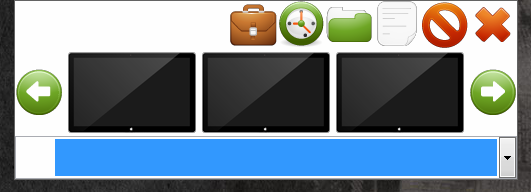
\includegraphics{screencap.png}
\caption{The UI of Chimaira; Several icons for different functions.}\end{figure}

The screen icons identify different screens nodes. The user can drop files on to these icons, causing the dropped files to be opened in the specific node. The arrows control the carousel of nodes, and are visble only if more than three nodes are connected. The drop-down list in holds recently viewed files in the selected project.


\begin{threeparttable}
\capstart\caption{Icons explained}

\begin{tabulary}{\linewidth}{|L|L|}
\hline
\textbf{
Icon
} & \textbf{
Description
}\\\hline

Briefcase
 & 
Select a project
\\\hline

Clock
 & 
Start / End a session
\\\hline

Folder
 & 
Open project directory
\\\hline

Note
 & 
Create an Event note
\\\hline

Circle
 & 
Hide the application
\\\hline

Cross
 & 
Exit the application
\\\hline
\end{tabulary}

\end{threeparttable}



\chapter{Indices and tables}
\label{index:indices-and-tables}\begin{itemize}
\item {} 
\emph{genindex}

\item {} 
\emph{modindex}

\item {} 
\emph{search}

\end{itemize}


\renewcommand{\indexname}{Python Module Index}
\begin{theindex}
\def\bigletter#1{{\Large\sffamily#1}\nopagebreak\vspace{1mm}}
\bigletter{c}
\item {\texttt{controller}}, \pageref{api:module-controller}
\indexspace
\bigletter{m}
\item {\texttt{models}}, \pageref{api:module-models}
\indexspace
\bigletter{s}
\item {\texttt{swnp}}, \pageref{api:module-swnp}
\indexspace
\bigletter{u}
\item {\texttt{utils}}, \pageref{api:module-utils}
\indexspace
\bigletter{w}
\item {\texttt{wos}}, \pageref{api:module-wos}
\end{theindex}

\renewcommand{\indexname}{Index}
\printindex
\end{document}
